Given the recorded SPIM observations $\phi_\nu$ of a geometric volume for each angle $\nu$ (also referred to as \textit{view}), the current deconvolved estimate $\psi^{r+1}$ for iteration $r+1$ is given by (in a very general form):\newline

\begin{equation}
\psi^{r+1} = \psi^{r} \prod_{\nu \in V} \frac{\phi_{\nu}}{\psi^{r} \ast P_{\nu} } \ast P^{compound}_{\nu}
\label{iterative_deconv}
\end{equation}

Here, $P_{\nu}$ refers to the experimentally obtained optical point-spread function (PSF) for angle $\nu$. $\ast$ denotes the discrete convolution, i.e. given an image $f$ and a convolution kernel $g$ the convolution of the two would be given by $f \ast g$. $P^{compound}_{\nu}$ denotes a compound point spread function over virtual views calculated from all $P_{\nu}$. The interested reader is hereby referred to \cite{2013arXiv1308.0730P} for the derivation and further details that lead to and explain equation \ref{iterative_deconv}.\newline

The implementation of the above was performed in java \cite{fiji_wiki_mvd} and is available as a plugin to the fiji image analysis platform \cite{fiji_website}. The core algorithm can be described in pseudo-code as in listing \ref{lst:java_implementation}.\newline

\begin{lstlisting}[caption={Java Implementation of Multi-View Deconvolution.},label={lst:java_implementation}]
stack_f32 psi = stack_f32(const);
stack_f32 view[n_view], kernel1[n_view],     //loaded from disk
	  kernel2[n_view], weights[n_view];  //loaded from disk

for( i : n_iterations ){
  for( v : n_view ){
    stack_f32 temp = psi;
    temp = convolve(temp,kernel1[v]);	    
    temp = view[v]/temp;
    temp = convolve(temp,kernel2[v]);	    
    psi = regularize(psi, temp, weights);
  }
}
\end{lstlisting}

In listing \ref{lst:java_implementation}, \texttt{stack\_f32} refers to a type that describes a three dimensional image where each intensity is encoded as a 32-bit floating point number. Related to this, the C/C++ array notation is used to indicate that each run of the deconvolution requires all image views \texttt{stack\_f32 view[n\_view]}, all per-view PSFs \texttt{kernel1[n\_view]}, all compound PSFs \texttt{kernel2[n\_view]} and all weight distributions \texttt{weights[n\_view]} to be available in memory. \texttt{psi} notes the deconvolved view that is updated by each iteration of the double loop in line $4-5$. The function call \texttt{convolve} denotes the convolution described in equation \ref{iterative_deconv} as $\ast$. The regularization mentioned in listing \ref{lst:java_implementation} has been omitted from equation \ref{iterative_deconv} for the sake of clearity, but is further described in the corresponding paper \cite{2013arXiv1308.0730P}. Any padding to the input \texttt{view} and \texttt{weights} as well as embedding of both PSFs into zero-filled images of the same shape as \texttt{view} is omitted from listing \ref{lst:java_implementation} also for readability. \newline

\begin{figure}[h]
  \centering
  \hfill
  \begin{subfigure}[b]{0.3\textwidth}
    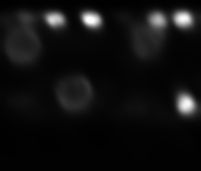
\includegraphics[width=\textwidth]{img/janosch_celegans_DAPI_nuclei_it1}
    \caption{start}
    \label{fig:iterate_start}
  \end{subfigure}%
  \hfill
  \begin{subfigure}[b]{0.3\textwidth}
    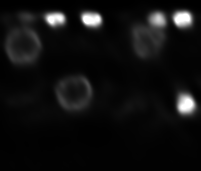
\includegraphics[width=\textwidth]{img/janosch_celegans_DAPI_nuclei_it3}
    \caption{iteration $2/5$}
    \label{fig:iterate_2}
  \end{subfigure}
  \hfill
  \hfill
  \begin{subfigure}[b]{0.3\textwidth}
    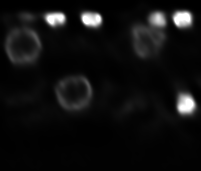
\includegraphics[width=\textwidth]{img/janosch_celegans_DAPI_nuclei_it5}
    \caption{iteration $5/5$}
    \label{fig:iterate_final}
  \end{subfigure}
  \hfill
  \caption{C. Elegans embryo data contrast improvements from multi-view deconvolution after no (figure \ref{fig:iterate_start}), after $2$ (figure \ref{fig:iterate_2}) and after $5$ iterations (figure \ref{fig:iterate_final}). }
  \label{fig:mvdeconv}
\end{figure}

Figure \ref{fig:mvdeconv} underlines the dramatic contrast improvements that \texttt{Multi-View Deconvolution} can yield. The data used this experiment was obtained from a commercial system, the Carl Zeiss Lightsheet Z.1, \cite{lz1}. 

\begin{table}[bht]
  \label{typ_datasets}
  
  \begin{tabular}{ccc}                                                                                                                                                                              
    \hline                                                                                                                                                                                         
    View Shape  & Number of Views and Channels & Data Volume [MB]   \\
    \hline                                                       
    $928\times390\times390$ & $6 \times 1$ & $807$ \\
    $1670\times1070\times345$ & $4 \times 2$ & $4703$ \\
    $1920\times1920\times320$ & $5 \times 1$ & $5625$ \\
    \hline                                                                                                                                                                                         
  \end{tabular} 
  \caption{Typical SPIM dataset shapes, number of views and color channels (per view). All datasets save the pixel intensity as 16-bit integer value. The latter has been used to calculate the raw data set volume.}
\end{table} 

In order to set the implementation to scale, table \ref{typ_datasets} lists typical data sets from SPIM instruments. It is important to note that the majority of instruments store the image data as 16-bit integer value. The PSF used for the deconvolution are obtained programmatically from sub-resolution beads distributed throughout the recorded volume inside the data set. Their sizes range are e.g. $79 \times 121 \times 101$ (obtained from the same data set that was used for figure \ref{fig:mvdeconv}). In order to save computations, the PSFs are truncated in practise $21 \times 21 \times 25$. \\

As the algorithm at hand relies twice on convolutions, this operation is deemed to be the largest consumer of run time. A convolution is a filtering operation, that operates on and n-dimensional image $f$ and convolves it by a filter kernel $g$ of similar or less dimensionality. Assuming that $f$ and $g$ are three-dimensional pixel collections and that $g$ has dimensions $N_{x} \times N_{y} \times N_{z}$, a convolution for an output pixel at location $[x,y,z]$ is calculated as 

\begin{equation}
  \label{eq:disc_convolve}
  (f \ast g)[x,y,z] = \sum^{i_x = N_{x}/2}_{i_x = -N_{x}/2} \sum^{i_y = N_{y}/2}_{i_y = -N_{y}/2} \sum^{i_z = N_{z}/2}_{i_z = -N_{z}/2} f[x-i_x,y-i_y,z-i_z] \cdot g[i_x,i_y,i_z].
\end{equation}

This operation does not only yield complications towards the borders of $f$ where $f[x-i_x,\dots]$ may refer to a pixel location outside the actual image (i.e. of unknown intensity), it is moreover of complexity 

\begin{equation}
\label{eq:discrete_convol_complexity}
\mathcal{O}(F[f \ast g]) = \mathcal{O}(I_{x} I_{y} I_{z} N_{x} N_{y} N_{z})
\end{equation}


where $I_{n}$ refers to the extent of $f$ in dimension $n$. Given the datasets listed in table \ref{typ_datasets}, this is an computationally expensive operation. As the convolution per output pixel $(f \ast g)[x,y,z]$ is independent of the calculation of every other output pixel $(f \ast g)[x',y',z']$, a convolution might at first glance yield high speed-ups when implemented on GPGPUs. As discussed in \cite{eklund_nonseparable_filtering}, this is only true for small kernel sizes on the order of $6 \times 6 \times 6$ at a fixed input image size. This is due to the fact that 2 arithmetic operations for every 2 arithmetic operations have to be performed. This results in an arithmetic complexity (number of arithmetic operations divided by the number of memory loads) of $1$. This has long been known \cite{massively_parallel_book} to be a regime, where GPGPUs do not perform well. To mitigate this short coming, the convolution theorem (equation \ref{}) can be exploited which states that a convolution in the spatial domain can be performed as a multiplication in the frequency domain.

\begin{equation}
  \label{eq:convol_theorem}
  F[f \ast g] = F[f] \cdot F[g]
\end{equation}

Here, $F[f]$ gives the Fourier Transform of $f$ into the frequency domain and $\cdot$ notes the element-wise multiplication of $F[f]$ and $F[g]$. The implementation of fast Fourier Transforms (FFT) has been studied for more than 50 years by now \cite{FFTCooleyTurkey,FFTBluestein,FFTRaders}. For the purpose of convolution, the complexity of the algorithm is hence reduced to 

\begin{equation}
  \label{eq:fft_convol_complexity}
  \mathcal{O}(F[f] \cdot F[g]) = 2\times\mathcal{O}(I\log I) + \mathcal{O}(I) = \mathcal{O}(I\log I)
\end{equation}

Here, $I = I_{x} \cdot I_{y} \cdot I_{z}$ refers to the total number of pixels in image $f$. As the FFT is performed on non-complex data further simplifications can be applied to it's implementation which renders equation \ref{eq:fft_convol_complexity} to be an upper bound rather than an exact value as in equation \ref{eq:discrete_convol_complexity}. The library as the result of the discussion at hand interfaces to the \texttt{fftw} (\cite{FFTW05}) library which contains highly optimised FFT implementations performed on the Central Processing Unit (CPU). The CPU-based implementation of the multi-view deconvolution is based on listing \ref{new_implementation}.

\clearpage

\begin{lstlisting}[caption={Optimized CPU Implementation of Multi-View Deconvolution. All FFT are explicitely stated \texttt{fft} as well as the corresponding normalized inverse operations \texttt{ifft}. },label={lst:new_implementation}]
stack_f32 psi = stack_f32(const);
stack_f32 view[n_view], kernel1[n_view],     //loaded from disk
	  kernel2[n_view], weights[n_view];  //loaded from disk

for( v : n_view ){
  kernel1[v] = fft(kernel1[v]);
  kernel2[v] = fft(kernel2[v]);
}

for( i : n_iterations ){
  for( v : n_view ){
    stack_f32 temp = psi;
    temp = ifft(fft(temp)*kernel1[v]);
    temp = view[v]/temp;
    temp = ifft(fft(temp)*kernel2[v]);
    psi = regularize(psi, temp, weights);
  }
}
\end{lstlisting}

Listing \ref{lst:new_implementation} contains one central improvement over listing \ref{lst:java_implementation}, whereby the FFT of \texttt{kernel1} and \texttt{kernel2} is performed before the iterative double loop is entered. This removes $n_{iterations}\cdot n_{view}$ executions of a FFT of size $I$ from the algorithm, which is beneficial not only in terms of runtime but also in terms of the memory budget.

For the GPGPU implementation interfacing to the \texttt{cufft} library (\cite{cufft}), the CPU implementation is used as a reference for code validation.
